\documentclass[10pt,twocolumn,a4paper]{article}
\usepackage[latin1]{inputenc}
\usepackage{amsmath}
\usepackage{amsfonts}
\usepackage{amssymb}
\usepackage{tikz}
\usepackage{listings}
\usepackage[width=17.00cm]{geometry}
\usepackage{graphicx}
\graphicspath{{./images/}}
\newcommand{\argt}{\theta}



\title{\LARGE{\textbf{Proyecto 2020} \\
		
		
		
		 ASIGNATURA \; \; \; LIC MI CARRERA\\
	
	
	
	\textbf{Orientaciones metodol\'ogicas:\\} Este es el tema de mi clase\\}

Estudiante P\'erez P\'erez \footnote{Soy estudiante de X a�o de mi carrera.}\\}
\date{}
%\renewcommand{\baselinestretch}{1.4}
\renewcommand{\labelenumi}{\alph{enumi}.}

\newtheorem{eje}{Ejercicio}
\newcommand{\sen}{\mbox{sen \hspace{0.001cm}}}
\newcommand{\cis}{\hspace{0.5mm}\mbox{cis}\hspace{0.5mm}}
\newcommand{\real}{\mathbb{R}}
\newcommand{\complex}{\mathbb{C}}




\begin{document}
\maketitle
\setcounter{page}{1}


\section*{Ejercicios}
\begin{eje}
    Genere una Poblaci�n normal de tama�o 500, seleccione 8 muestras de tama�os varios(Muy mayor que 30, mayor que 30, 30, 20), 4 muestras con remplazo y 4 sin remplazo.
    \begin{enumerate}
        \item Calcule para cada una de las muestras los Estad�sticos Descriptivos, de la Conferencia 1.
        \item Calc�lelos en la poblaci�n inicial. Analice las diferencias.
        \item Grafique los resultados.
        \item Para cada muestra calcule los intervalos de confianza para la media y la varianza.
        \item Analice las diferencias en los resultados de las muestras de tama�os similares.
    \end{enumerate}
	Propuesta de distintos ejercicios de la clase, para desarrollar las habilidades a crear durante la clase.
\end{eje}
\begin{eje}
	De acuerdo a su set de datos(Equipo 10):
	\begin{enumerate}
			\item Utilice los Estad\'isticos Descriptivos estudiados en la Conferencia 1. Para describir el comportamiento de tres de sus variables. Seleccione las que sean m\'as importantes y explique porque seleccion\'o estas.
			\item Grafique los resultados.
			\item Interprete los resultados en t\'erminos del problema.
	\end{enumerate}
\end{eje}
\begin{eje}
    Analizando los datos del archivo "adult.data.csv"(Equipo 10), �Hay diferencias significativas entre el promedio de a�os dedicados a la educaci�n y la cantidad de ingreso de los censados?
\end{eje}


\section*{Objetivos}
\begin{itemize}
	\item Aprender sobre el trabajo con los estad\'isticos descriptivos, estimaci\'on y prueba de hip\'otesis. 
	\item Ganar experiencia en el trabajo con el lenguaje R. 
\end{itemize}
 
\section*{Introducci\'on} 

En este proyecto se ponen en pr\'actica el uso y comparaci\'on con estad\'isticos descriptivos  en poblaciones y muestras generadas con el lenguaje de programaci\'on R. Tambi\'en se trabaja con un conjunto de datos reales. En este caso, se trata de analizar el ingreso anual de un conjunto de individuos y caracterizar las variables que se consideran m\'as importantes para el problema. Para ello se hacen pruebas de hip\'otesis y se usan gr\'aficos de cajas e histogramas para mostrar los resultados, auxiliandose del lenguaje R.
		


\section*{Ejercicio 1}
\textit{(c\'odigo referente al ejercicio en exercise\_1.R)}
 %(Zmin')
 
\subsection*{Diferencias entre las muestras y la poblaci\'on}

Se genera una poblaci\'on inicial con 500 elementos y una distribuci�n normal con media 0 y varianza 1. Luego se extraen 4 muestras sin remplazo, cada una de tama�o 200, 60, 30 y 20 respectivamente. Luego se extraen otras 4 de igual tama�o a las anteriores y con remplazo. Para cada muestra se calculan media, mediana, varaiaci\'on y desviaci\'on est\'andar. Los datos son continuos y la probabilidad de que 2 datos sean iguales es teoricamente 0, por ende asumimos que la moda nunca existe.

La exactitud de los estimadores puntuales fluctua en cada prueba realizada, la fluctuaci\'on es mayor o menor dependiendo del tama\~no de las muestras.\\
Las muestras de mayor tama�o presentan estimadores m�s exactos, en cambio, las de menor tama�o suelen estar m�s alejadas del valor real.
Esto se debe a que en las muestras m�s grandes cuando tienen un caso extremo no representativo de la poblaci�n su impacto queda disminuido por el resto de los datos no extremos,
mientras que en las muestras peque�as la existencia de uno de estos altera considerablemente la informaci�n extra\'ida.

Queda reflejada entonces una dependencia directa que existe entre los resultados de una muestra y la calidad de sus datos. Podemos deducir entonces la importancia de que las muestras esten compuestas por datos fiables, incluso m\'as cuando la muestra es peque\~na.\\

Para visualizar los resultados utilizamos un gr\'afico de cajas y bisagras y gr\'aficos de barras. El primero por su propiedad para dar en una sola imagen percentiles, mediana, m\'inimo y m\'aximo, adem\'as si las partes de las cajas se encunetran simetricas y centrada en los datos indica que estos siguen una dsitribuci\'on normal. El gr\'afico de barras lo utilizamos para visualizar las diferencias de la media y la varianza en las distintas muestras y poblaci\'on.

Como ejemplo, en la figura\footnote{Posible visualizar en mayor detalle cuando se ejecute el c\'odigo.} se puede apreciar un gr\'afico de cajas y bigotes distribuidos consecutivamente, donde cada gr\'afico corresponde a una muestra distinta. La caja de las muestras de tama\~no 200 se encuentran generalmente alineadas y bien formadas, indicador de que sus datos mantienen la distribuci�n normal de la poblaci\'on de la cual fueron extra\'idos.
La representaci\'on de las otras muestras puede estar bien formadas o no.
En este ejemplo es posible ver que las muestras peque\~nas la caja esta deformada por lo que sus datos no son representativos de la poblaci\'on,
al igual que la muestra de tama�o 60 sin remplazo, mientras que la muestra de tama\~no 60 con remplazo sus datos est\'an relativamente alineados con los de la poblaci\'on.

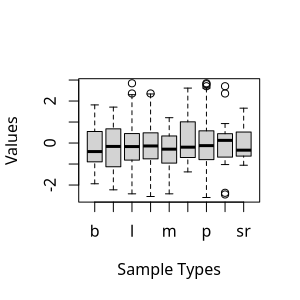
\includegraphics{images/ex1_box_300.png}
\textit{p: poblaci\'on, l: muestra de tama\~no 200, b: tama\~no 60, m: tama\~no 30 y s: tama\~no 20}.
\textit{Si tiene r al final es muestra con remplazo}

\subsection*{Intervalos de Confianza y diferencias entre las muestras de igual tama\~no}
Se estiman los intervalos de confianza para la media y la varianza con un nivel de signifaci\'on del 5 por ciento. Luego se comparan los resultados entre las muestras de mismo tama�o.

Durante todas las pruebas realizadas todos los intervalos de confianza fueron correctos, es decir, la media y la varianza de la poblaci\'on siempre estuvieron dentro de los intervalos calculados.
La diferencia m\'as notable que ocurri\'o de manera consistente en todas las pruebas realizadas fue la diferencia de tama\~no en los intervalos entre las muestras con mayor cantidad de datos y menor cantidad respectivamente. Una muestra con menor cantidad de datos resulta en un intervalo de confianza m\'as amplio.

Durante nuestras pruebas no hubo una diferencia notable en los intervalos de confianza entre las muestras extraidas con remplazo y sin remplazo.

\subsection*{Conocimientos adquiridos}
Podemos decir a modo de an\'alisis final que el proceso de obtener una muestra no basta solo con recoger datos aleatorios, es importante que los datos sean representativos de la poblaci\'on. En caso de que no se tenga informaci\'on sobre la poblacion obtener la mayor cantidad de datos posibles.

Tambien visaulizamos como las f\'ormulas estudiadas se adapantan y complementan para dar un resultado correcto. En el caso de las muestras de mayor cantidad de datos sus estimadores puntuales usualmente son m\'as exactos que en las muestras peque\~nas y estas \'ultimas en consecuencia tienen un intervalo de confianza de mayor tama�o como compensaci\'on a la inexactitud de sus estimadores puntuales.

\section*{Ejercicio 2} 
\textit{El c\'odigo referente a este ejercicio esta en el archivo exercise\_2.R}\\

El dataset contaba con valores faltantes. Para lidiar con este problema se realiz\'o un preprocesamiento de los datos. Se ten\'ian dos opciones: descartar dichos valores faltantes o sustituirlos por la media de los conocidos. Se opt\'o por la \'ultima opci\'on. De esta forma se obtuvo un conjunto de datos m\'as limpio y completo que facilit\'o el trabajo en el posterior an\'alis.

Como parte del an\'alisis se tomaron tres variables que se consideraron las m\'as importantes. Primeramente tomamos 'education', pues consideramos que el nivel de educaci\'on influye en gran medida en el salario de una persona. No suelen ganar lo mismo una persona con nivel universitario que una que solamente tiene un nivel medio-superior. La otra variable escogida para analizar fue 'occupation'. El salario de una persona est\'a determinado principalmente por su profesi\'on o el tipo de trabajo que realiza. Como tercera y \'ultima  variable a analizar se tom\'o 'sex'. Se decidi\'o tomar esta variable porque se sabe que en la actualidad todav\'ia existen diferencias en cuanto al salario de dos personas que  realizan el mismo trabajo en dependencia del sexo, por lo que resulto de inter\'es trabajar con esta variable.

Para garantizar la veracidad de los planteamientos  anteriores se hicieron pruebas de hip\'otesis para cada uno de estos atributos. El resultado coincidi\'o. Tanto la educaci\'on como la ocupaci\'on y el sexo influyen significativamente en los ingresos anuales de una persona. Sin embargo, se decidi\'o analizar el resto de variables y se pudo observar un hecho interesante: la gran mayor\'ia de los atributos del dataset influyen significativamente en los ingresos anuales de una persona. Por lo que podemos decir que se hizo una muy buena selecci\'on de variables a la hora de recopilar informaci\'on referente al problema.

Con respecto a los resultados obtenidos a trav\'es del an\'alisis descriptivo de las tres variables escogidas, la tabla \ref{tab:table4} los muestra .En las figuras de la 1 a la 6 se muestran algunos resultados gr\'aficamente. En este caso, todas las variables escogidas eran categ\'oricas por lo que se codificaron en valores enteros. En las tablas \ref{tab:table1},\ref{tab:table2} y \ref{tab:table3}   se puede apreciar que valor representa cada n\'umero.

\subsection*{ Interpretaci\'on de los resultados }

En el caso de la ocupaci\'on la mediana fue 6( Exec-managerial ) , lo que implica que la mayor parte de  individuos (50\%) que forman parte de la muestra se dedican a esta ocupaci\'on. La moda fue tambi\'en 6, lo cual significa que es la ocupaci\'on a  que m\'as se repite entre los individuos de la muestra. El valor del coeficiente de variaci\'on es de 48\% aproximadamente, por tanto los datos son muy heterog\'eneos. 

En el caso de la educaci\'on la mediana fue 4 (HS-grad), lo cual indica que alrededor del 50\% de los individuos tienen al menos nivel medio superior. La moda tambi\'en fue 4, lo cual implica que la mayor parte de las personas ten\'ian  nivel medio superior en cuanto a educaci\'on. Por \'ultimo, el valor del coeficiente de variaci\'on es de 86\% aproximadamente por lo que los datos son muy heterog\'eneos. 

Finalmente, para el sexo, se obtuvo  que la mediana y el la moda tomaron el mismo valor: 2. Eso implica que los valores intermedios de los datos son de sexo masculino , y que  estos individuos  son los que tienen mayor presencia en el dataset.

\begin{table}[h!]
  \begin{center}
    \caption{Valores num\'erico de las categor\'ias de educaci\'on }
    \label{tab:table1}
    \begin{tabular}{|l|c|} 
		\textbf{Categor\'ia} & \textbf{Valor} \\
		Bachelors   &1 \\
	    Some-college&2 \\
		11th        &3 \\
		HS-grad     &4 \\
	    Prof-school &5 \\
		Assoc-acdm  &6 \\
		Assoc-voc   &7 \\
		9th         &8 \\
	    7th-8th     &9 \\
		12th        &10 \\
		Masters     &11 \\
		1st-4th     &12 \\
		10th        &13 \\
		Doctorate   &14 \\
		5th-6th     &15 \\
		Preschool   &16 \\
      \hline
    \end{tabular}
  \end{center}
\end{table}

\begin{table}[h!]
  \begin{center}
	  \caption{Valores num\'ericos de las categor\'ias de ocupaci\'on }
    \label{tab:table2}
    \begin{tabular}{|l|c|} 
		\textbf{Categor\'ia} & \textbf{Valor} \\
		 Tech-support      &1 \\
		 Craft-repair      &2 \\
		 Other-service     &3 \\
		 Sales             &4 \\
		 Exec-managerial   &5 \\
		 Prof-specialty    &6 \\
		 Handlers-cleaners &7 \\
		 Machine-op-inspct &8 \\
		 Adm-clerical      &9 \\
		 Farming-fishing   &10 \\
		 Transport-moving  &11 \\
		 Priv-house-serv   &12 \\
		 Protective-serv   &13 \\
		 Armed-Forces      &14 \\
           \hline
    \end{tabular}
  \end{center}
\end{table}

\begin{table}[h!]
  \begin{center}
	  \caption{Valores num\'ericos de las categor\'ias de sexo  }
    \label{tab:table3}
    \begin{tabular}{|l|c|} 
		\textbf{Categor\'ia} & \textbf{Valor} \\
		  Femenino      &1 \\
		  Masculino      &2 \\
           \hline
    \end{tabular}
  \end{center}
\end{table}

\begin{table}[h!]
  \begin{center}
    \caption{}
    \label{tab:table4}
    \begin{tabular}{|l|c|c|c|} 
		\textbf{Estad\'igrafo} & \textbf{Ocupaci\'on} & \textbf{Educaci\'on} &\textbf{Sexo }\\
    Media &  6& 4  &2   \\
    Mediana & 6 &4  &2  \\
    Varianza & 8.35 & 11.98 &  0.22\\
    DS &2.89  & 3.46 & 0.47  \\
	CV &  0.48& 0.86 &0.23 \\
    Moda & 6  & 4 & 2 \\
	Min &1 &1 &1 \\ 
	Lower-Hinge &3 &2 &1 \\ 
	Median &6 &4 &2 \\ 
	Upper-Hinge &8 &5 &2 \\ 
	Max & 14&16 &2 \\ 
      \hline
    \end{tabular}
  \end{center}
\end{table}

\begin{figure}
    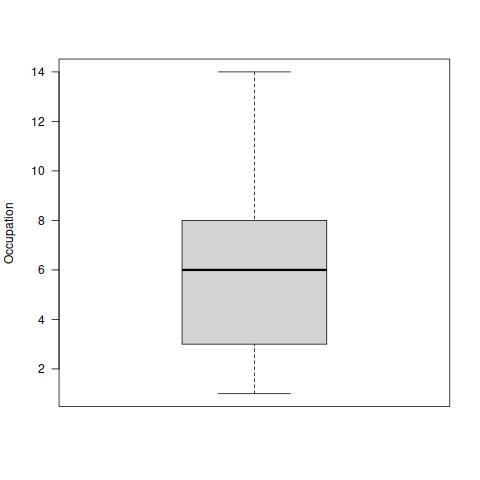
\includegraphics[width=\linewidth]{images/boxplot_occupation.jpeg}
    \caption{Boxplot para ocupaci\'on}
    \label{fig:boxplot_occupation}
\end{figure}

\begin{figure}
    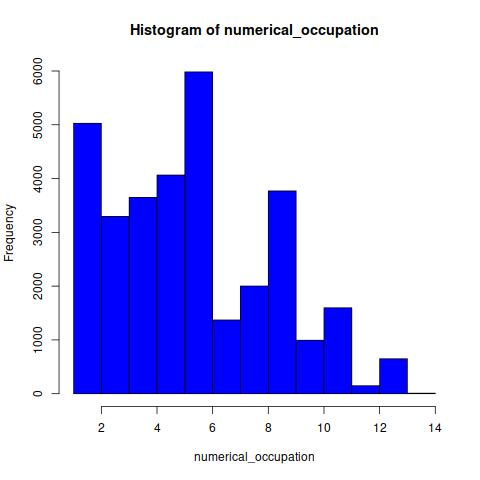
\includegraphics[width=\linewidth]{images/hist_occupation.jpeg}
    \caption{Histograma de ocupaci\'on}
    \label{fig:hist_occupation}
\end{figure}

\begin{figure}
    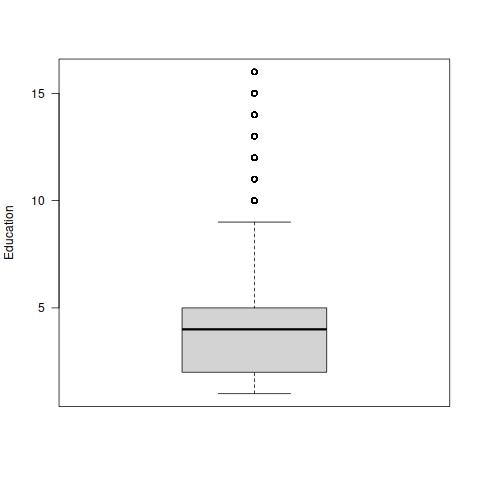
\includegraphics[width=\linewidth]{images/boxplot_education.jpeg}
    \caption{Boxplot para educaci\'on}
    \label{fig:boxplot_education}
\end{figure}

\begin{figure}
    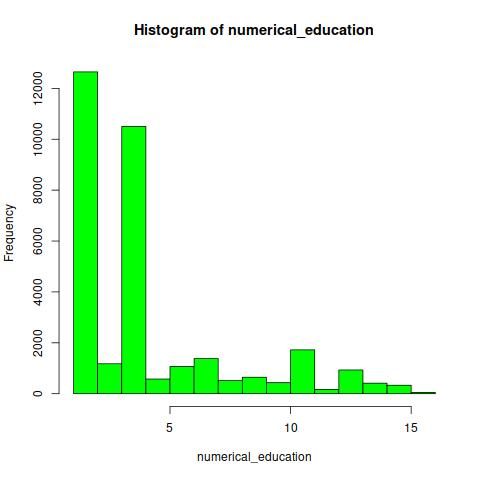
\includegraphics[width=\linewidth]{images/hist_education.jpeg}
    \caption{Histograma de educaci\'on}
    \label{fig:hist_education}
\end{figure}

\begin{figure}
    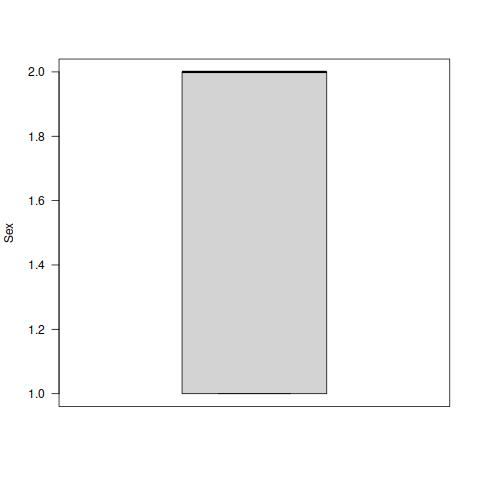
\includegraphics[width=\linewidth]{images/boxplot_sex.jpeg}
    \caption{Boxplot para sexo}
    \label{fig:boxplot_sex}
\end{figure}

\begin{figure}
    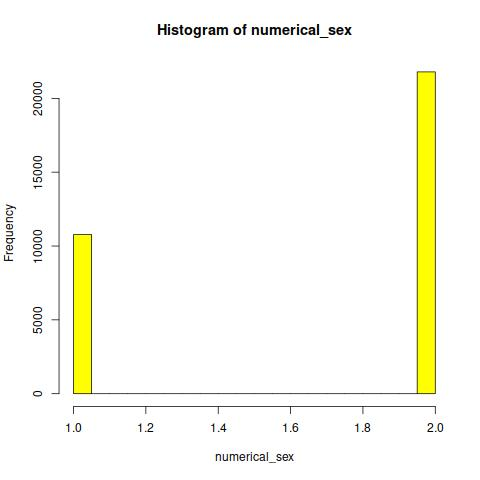
\includegraphics[width=\linewidth]{images/hist_sex.jpeg}
    \caption{Histograma de sexo}
    \label{fig:hist_sex}
\end{figure}


\section*{Ejercicio 3}
El problema trata sobre comparar la medias de a�os de educacion de los grupos de ingresos $\le50K$ y $>50K$, y ver si hay alguna diferencia significativa entre esas medias.\\
\textit{El c\'odigo referente a este ejercicio esta en el archivo exercise\_3.R}\\
Para lograr lo anterior se dividi\'o todos los datos del archivo csv en dos grupos: un grupo tiene ingresos $\le 50K$ y otro grupo tiene ingresos de $>50K$.\\
Luego de realizar la divisi\'on se escogieron dos muestras sin reemplazo de tama\~no $N= 60$ cada una.\\
Por lo que el problema se reduce a una prueba de hip�tesis para la comparaci�n de las medias de dos poblaciones Normales.\\
Las hip\'otesis para la prueba que se escogieron fueron:
$$
	H_0: \mu_1 = \mu_2
$$
$$
	H_1: \mu_1 \ne \mu_2
$$
Donde $\mu_1$ es la media de a\~nos de educaci\'on de la poblaci\'on de personas que poseen ingresos por debajo de los $50K$(inclusivo) y $\mu_2$ es la media de a\~nos de educaci\'on de la poblaci\'on de personas que poseen ingresos por encima de los $50K$.\\
Se asumi\'o que no se conoc\'ian las varianzas de dichos grupos(o que era muy costoso calcularlas). Por lo que para hacer la prueba de hip\'otesis de la media se hace primero una prueba de hip\'otesis para la igualdad de las varianzas.

\begin{lstlisting}[language=R,title=Parte del codigo para la hipotesis de varianza]
result <- var.test(sample1,
sample2, alternative = "two.sided")
\end{lstlisting}

Luego de establecer la igualdad o desigualdad de varianza se procede a realizar la prueba de la media:

\begin{lstlisting}[language=R,title=Parte del codigo para la hipotesis de la media]
result <-t.test(sample1,sample2, 
alternative = alt, var.equal = varequal)
\end{lstlisting}

Finalmente se compara el resultado del \textit{p-value} de \textit{result} con un valor $\alpha$ preestablecido y si es menor se rechaza la hip\'otesis nula.

\subsection*{Anal\'iticamente}
Se hace primero la prueba de varianza.\\
Los datos se tomaron del script referente al ejercicio.\\
$H_0: \sigma_1^2 = \sigma_2^2$\\
$H_1: \sigma_1^2 \ne \sigma_2^2$\\
$$
F = \frac{S_1^2}{S_2^2} = \frac{6.37}{5.13}= 1,24
$$
	$$
F_{1- \alpha /2}(n_1  - 1, n_2 - 1) = F_{0.975}(59,59) = 1.67
$$
$$
F_{\alpha/2}(n_1 -1, n_2-1) = F_{0.025}(59,59) =0.597
$$
Como $F> 	F_{\alpha/2}(n_1 -1, n_2-1)$ y $F< F_{1- \alpha /2}(n_1  - 1, n_2 - 1)$ no se puede descartar $H_0$ por lo que se asume que $\sigma_1^2 = \sigma_2^2$\\
$$
T_{\bar{X} - \bar{Y}} =	\frac{\bar{X} - \bar{Y}}{\sqrt{ (n_1 - 1)S_1^2 + (n_2 - 1)S_2^2   }}
\sqrt{\frac{n_1n_2(n_1+n_2-2)}{n_1 + n_2}} =3.7
$$
$$
t_{1-\alpha/2}(n_1+ n_2 -2) = t_{0.975}(116) =1.98
$$
Como $|T_{\bar{X} - \bar{Y}}| > t_{1-\alpha/2}(n_1+ n_2 -2)$ se cumple la regi\'on cr\'itica y se descarta $H_0$ pudiendo afirmarse que se aprecian diferencias significativas.



\section*{Conclusiones}


Mediante los m\'etodos abordados en el proyecto se pueden describir caracter\'isticas de las poblaciones para lograr un mejor entendimiento de lo que se tiene en una determinada situaci\'on. Adem\'as, podemos estimar par\'ametros de la poblaci\'on que no conocemos para lograr predecir comportamientos o eventos. Tambi\'en podemos comparar dos tipos de poblaciones por sus param\'etros y llegar a conclusiones sobre que variables afectan m\'as un determinado resultado que estamos estudiando.


\section*{Conclusiones}

Mediante los m\'etodos abordados en el proyecto se pueden describir caracter\'isticas de las poblaciones para lograr un mejor entendimiento de lo que se tiene en una determinada situaci\'on. Adem\'as, podemos estimar par\'ametros de la poblaci\'on que no conocemos para lograr predecir comportamientos o eventos. Tambi\'en podemos comparar dos tipos de poblaciones por sus param\'etros y llegar a conclusiones sobre que variables afectan m\'as un determinado resultado que estamos estudiando.

\section*{Contribuciones de cada integrante}
Para la realizacion del proyecto se sigui\'o la siguiente estrategia:
\begin{itemize}
	\item Un integrante escoge uno de los tres ejercicios y lo soluciona.
	\item Luego de solucionarlo, el integrante le explica el ejercicio a los otros dos integrantes y \'estos a su vez act\'uan como adversarios y tratan de encontrarle alg\'un fallo en el c\'odigo o alguna explicaci\'on del informe que no est\'e muy clara.
\end{itemize}

Siguiendo esa estrategia los ejercicio se esogieron de la siguiente manera:
\begin{itemize}
	\item Rodrigo Pino el ejercicio 1.
	\item Adrian Portales el ejercicio 2.
	\item David Guaty el ejercicio 3.
\end{itemize}

  
\end{document}
